\chapter{Approccio proposto}
\label{chap:approccio}
\vspace{1cm}
Nel Capitolo \ref{chap:SOA} sono state descritte alcune soluzioni proposte 
relative al lavoro oggetto di questa tesi, in particolare algoritmi esatti ed
euristici di ottimizzazione basati su varie tecniche.
% TODO & FIXME aggiungere qualcosa (tipo pro/contro)

In questo capitolo verrà descritto l'approccio utilizzato per risolvere il 
problema di scheduling dei task tenendo in considerazione le comunicazioni e 
riconfigurazioni introdotte.

Il capitolo è organizzato secondo la seguente struttura: nella Sezione 
\ref{sec:integrazioneToolchainFASTER} viene descritta l'integrazione 
dell'algoritmo di scheduling con il componente che gestisce il mapping dei task, 
con accenni alle interfacce esterne che collegano il componente 
con gli altri strumenti utilizzati nella toolchain di \acs{FASTER}; la Sezione 
\ref{sec:panoramicaMetodologia} descrive  ad alto livello il funzionamento 
dell'algoritmo di scheduling, fornendo una panoramica delle fasi in cui questo 
si divide; la Sezione \ref{sec:euristicaSceltaTask} contiene una descrizione 
dettagliata della fase più delicata del procedimento di scheduling, la scelta 
del task migliore da considerare ad ogni passo di decisione; la Sezione 
\ref{sec:osservazioniConclusive} fornisce un riepilogo dei concetti importanti 
presentati in questo capitolo.


\section{Integrazione nella toolchain di \ac{FASTER}}
\label{sec:integrazioneToolchainFASTER}

Come descritto nel precedente capitolo, l'obiettivo del progetto europeo 
\ac{FASTER} è fornire un framework per la sintesi ad alto livello di 
applicazioni, scritte in linguaggio di programmazione C, su vari dispositivi 
riconfigurabili; la toolchain che permette di realizzare questa sintesi è 
composta da varie fasi eseguite in sequenza. Ogni fase deve essere il più 
possibile self-contained, ovvero deve poter essere invocata separatamente e non 
deve avere nozioni sul funzionamento interno delle altre fasi.

Condizione necessaria perchè ciò accada è la definizione di specifiche 
interfacce per ogni strumento che deve essere invocato. Ad esempio, la fase di 
mapping ha la propria interfaccia di input e di output; lo scheduler 
(incapsulato nell'algoritmo evolvibile di esplorazione delle soluzioni) ha 
anch'esso una interfaccia di input e una di output, contenenti tutte 
le strutture dati necessarie per l'elaborazione e per la memorizzazione delle 
informazioni calcolate dall'algoritmo, rispettivamente. 

\begin{figure}
 \begin{center}
  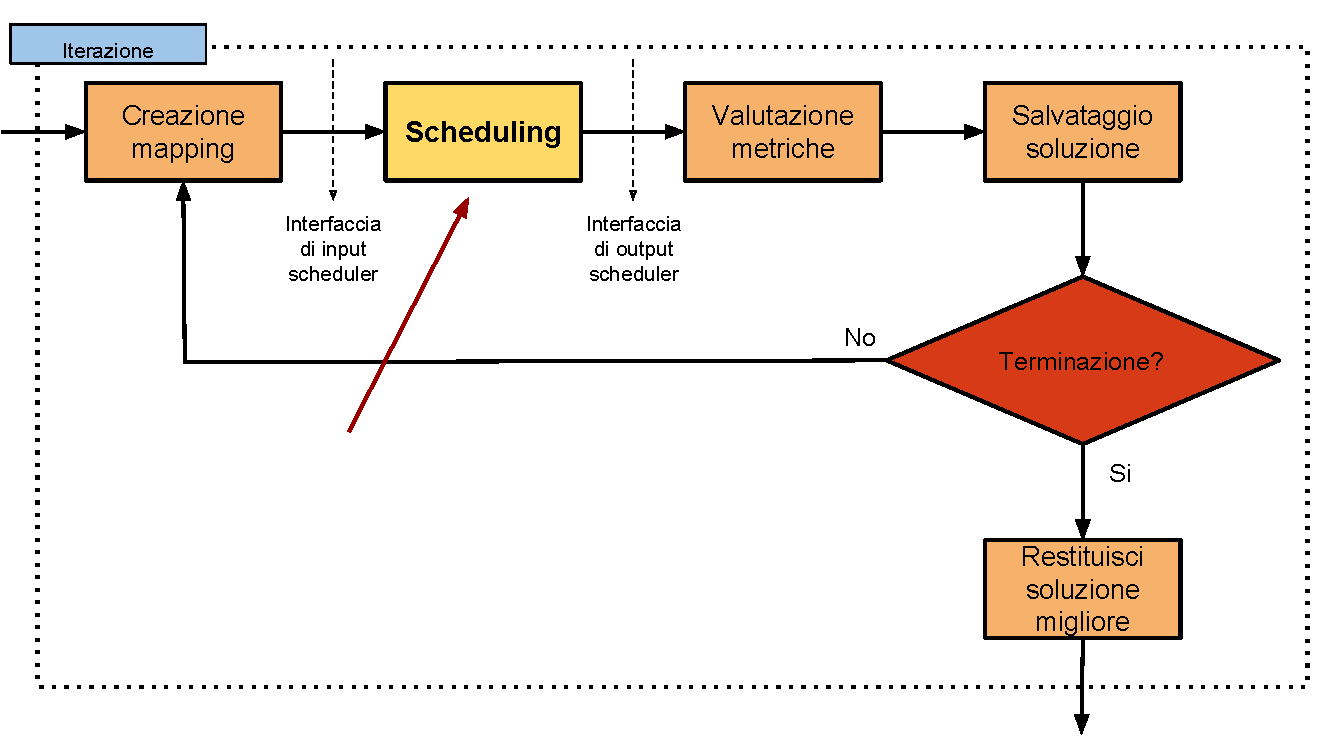
\includegraphics[width=0.9\textwidth]{capitoli/figure/cap3/MapperWorkflow.pdf}
  \caption{Flusso di lavoro dell'algoritmo di esplorazione.}
  \label{fig:mapperWorkflow}
 \end{center}
\end{figure}

A livello dell'algoritmo di esplorazione delle soluzioni, dunque, si avrà un 
flusso di lavoro come rappresentato nella Figura \ref{fig:mapperWorkflow}, in 
cui è messo in evidenza dove si colloca la fase di scheduling oggetto del 
lavoro, con le relative interfacce di input e output.

Anche la fase di mapping, che precede l'invocazione del tool che gestisce lo 
scheduling, è caratterizzata dalle proprie interfacce di input e output. Come 
si può vedere nella Figura \ref{fig:mapperWorkflow}, poichè la fase di 
scheduling è immediatamente successiva a quella di mapping, l'interfaccia di 
output del mapper e l'interfaccia di input dello scheduler avranno alcuni dati 
in comune.


\subsection{Interfaccia di input}

L'interfaccia di input per la fase di scheduling contiene tutti i dati 
necessari all'esecuzione dello scheduler, alcuni definiti prima 
dell'invocazione del tool, altri creati o modificati durante le differenti fasi 
dell'esecuzione. In particolare, i dati definiti prima dell'invocazione sono:
\begin{itemize}
 \item dati provenienti dal file XML di specifica del progetto correntemente in 
elaborazione dalla toolchain, relativi alla descrizione dell'architettura, del 
task graph, delle implementazioni e dei vari elementi di computazione, di 
comunicazione e di memoria presenti;
 \item dati provenienti dall'output della fase di mapping.
\end{itemize}

Questi ultimi sono organizzati come una lista di triple \emph{$<$processing 
task, processing element, implementazione$>$} calcolata dal mapper, che 
specifica per ogni task:
\begin{enumerate}
 \item l'elemento di computazione che dovrà eseguire il task, può essere un 
core hardware su scheda oppure un soft core (processore);
 \item l'implementazione da utilizzare per l'esecuzione del task, si può 
dividere in implementazione software o hardware a seconda che il task debba 
essere eseguito su scheda o su un processore.
\end{enumerate}
Le informazioni provenienti dal mapper vengono quindi utilizzate per 
determinare se alcune aree dovranno essere riconfigurate durante l'esecuzione 
dell'applicazione oppure no, oltre a dare informazioni sull'occupazione dei 
vari componenti del dispositivo.


\subsection{Interfaccia di output}




\section{Panoramica della metodologia}
\label{sec:panoramicaMetodologia}


\section{Euristica di scelta dei task}
\label{sec:euristicaSceltaTask}


\section{Osservazioni conclusive}
\label{sec:osservazioniConclusive}
